%%%%%%%%%%%%%%%%%%%%%%%%%%%%%%%%%%%%%%%%%%%%%%%%%%%%%%%%%%%%%%%%%%% 
%                                                                 %
%                         ACKNOWLEDGEMENT                         %
%                                                                 %
%%%%%%%%%%%%%%%%%%%%%%%%%%%%%%%%%%%%%%%%%%%%%%%%%%%%%%%%%%%%%%%%%%% 
 
\specialhead{PREFACE}
 
During my second year at RPI as an undergraduate, I began a research project with my current advisor, Professor Wilke, on the X-ray diffraction of montmorillonite clay samples. As a young aspiring physicist, I must admit that studying clay minerals was not high on my list of interests. That summer however, I was given a workbench in a chemistry lab, an assortment of various chemicals, and access to a very cool X-ray diffractometer. This mixture of excitement to begin using the diffractometer and pure fear of poisoning myself was an interesting feeling to say the least. As I began performing measurements and coming up with my first experiments, the fear subsided and I started to enjoy going to the lab, carrying a tray full of clay samples to the diffractometer, and spending several hours watching Bragg peaks form on a computer screen.

After that summer, I decided that looking at clay for the time being wasn't as odd or as boring as my parents initial reaction to hearing my research topic would have implied. I decided to keep working with Professor Wilke, who had a new experiment in mind for me, collecting infrared spectra of montmorillonite samples. My research in this field continued through my undergrad, until it became my graduate research as well, as I completed my Masters degree. After almost four years of working on a subject, you begin to acquire a large bit of knowledge and data on a topic. It is for this reason, and the fact that I desired to pursue my PhD in Europe, that Professor Wilke encouraged me to complete a Masters Thesis, in lieu of a Masters Project which is far more common in the Physics department. I was skeptical at first, as a thesis seemed like much more work than a project, and finishing a Masters degree in one year already seemed like it would be difficult enough. She insisted that I had enough work to produce a thesis, and that it would help me for when I have to write my Doctoral Thesis later on.

These seemed like valid reasons, so I followed her advice and opted for the thesis. As soon as I began writing this manuscript however, I realized that I had been right about something; writing a thesis is very difficult. The beginning was painfully slow, and the perpetual ignorance of not knowing where to even begin postponed its initiation. Once I had written my first chapter however, it started to become much easier to continue. I would find myself easily working until the early morning hours on the weekend, not realizing how much time had actually gone by. To a fair extent, I began to enjoy it. In addition, it was clear that I had learned a lot about the writing process, and also more about my research as a whole as I was forced to think about it in a new manner. This thesis has made me a better physicist, and better prepared me to go out, and begin work on a PhD. I cannot thank Professor Wilke enough for her encouraging me to complete a thesis, for without her advice this work would likely not exist, and I would not be as well prepared as I am today. To other young physicists reading this, I encourage you to do the same, as it will certainly make you a better scientist, and only better prepare you for the future, whether you plan on doing a PhD afterwords or not.
\newline
\begin{flushleft}
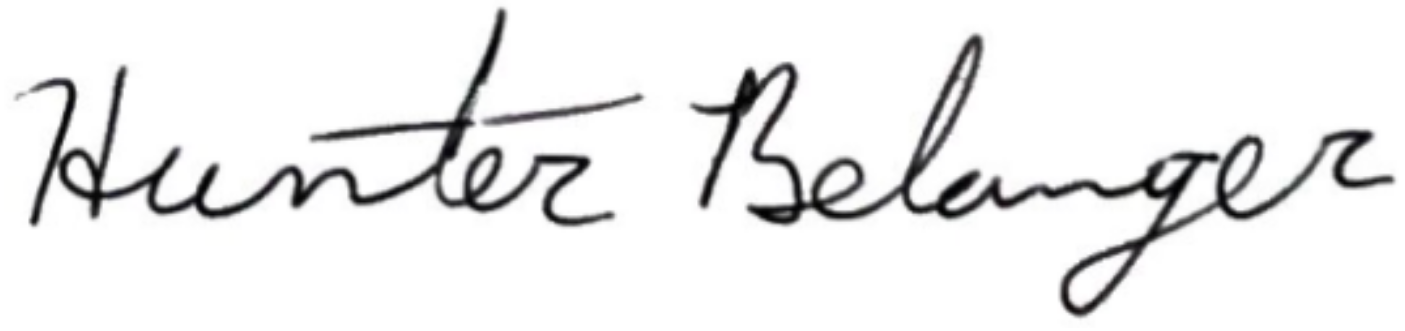
\includegraphics[scale=0.2]{images/signature.png}\newline
Hunter Belanger
\newline\newline
Troy, New York\newline
March, 2019
\end{flushleft}
